\documentclass[11pt,fleqn]{article}
\usepackage[a4paper,left=3cm,right=3cm,top=3cm,bottom=3cm]{geometry}
\usepackage{setspace}
	\onehalfspacing
	\setlength\parindent{0pt}
	\setlength\parskip{11pt}

\usepackage[american]{babel}
\usepackage[utf8]{inputenc}
\usepackage[T1]{fontenc}
\usepackage{lmodern}

\usepackage[round,authoryear]{natbib}
	\bibliographystyle{ecta}
\usepackage{titletoc}
\usepackage{hyperref}
	\hypersetup{colorlinks=true, linkcolor=blue, citecolor=blue, urlcolor=blue}
	
\usepackage{amsmath}
\usepackage{amssymb}
\usepackage{amsfonts}
\usepackage{mathtools}
\usepackage{dsfont}
	\newcommand{\id}{\mathds{1}}
\usepackage{accents}
	\newcommand{\barbelow}[1]{\underaccent{\bar}{#1}}
\usepackage{gensymb}
\usepackage{bm}

\usepackage{graphicx}
\usepackage{tikz}
	\usetikzlibrary{decorations.pathreplacing}
	\usetikzlibrary{decorations.shapes}
	\usetikzlibrary{arrows}
\usepackage{color}

\usepackage{url}
	\urlstyle{same}
\usepackage{enumerate}




% SPECIFIC SYNTAX

\newcommand{\N}{\mathbb{N}}
\newcommand{\R}{\mathbb{R}}

\renewcommand{\P}{\mathbb{P}}
\newcommand{\E}{\mathbb{E}}

\DeclareMathOperator*{\argmin}{\text{\normalfont arg\,min}}
\DeclareMathOperator*{\argmax}{\text{\normalfont arg\,max}}

\newcommand{\e}{\text{e}}

\newcommand\spiral{}% Just for safety so \def won't overwrite something
\def\spiral[#1](#2)(#3:#4:#5){% \spiral[draw options](placement)(end angle:revolutions:final radius)
\pgfmathsetmacro{\domain}{pi*#3/180+#4*2*pi}
\draw [#1,
       shift={(#2)},
       domain=0:\domain,
       variable=\t,
       smooth,
       samples=int(\domain/0.08)] plot ({\t r}: {#5*\t/\domain})
}






\begin{document}






% =========================================== %
% ++++++++++++++++ TITLEPAGE ++++++++++++++++ %
% =========================================== %

\date{\today}
\title{Homotopy Continuation}

\author{
Steffen Eibelshäuser\footnote{Goethe University Frankfurt, \href{mailto:eibelshaeuser@econ.uni-frankfurt.de}{\nolinkurl{eibelshaeuser@econ.uni-frankfurt.de}}} %
\and %
David Poensgen\footnote{Goethe University Frankfurt, \href{mailto:poensgen@econ.uni-frankfurt.de}{\nolinkurl{poensgen@econ.uni-frankfurt.de}}}
}

\maketitle
\thispagestyle{empty}

\noindent On the implementation of homotopy continuation in HomCont.

\vspace{2em}
\noindent HomCont: \\ Python software for solving systems of nonlinear equations \\ by homotopy continuation.

\vspace{4em}






% =================================================== %
% ++++++++++++++++ TABLE OF CONTENTS ++++++++++++++++ %
% =================================================== %

\begin{spacing}{0.75}
\tableofcontents
\thispagestyle{empty}
\end{spacing}
\vspace{4em}
\pagebreak






% ====================================== %
% ++++++++++++++++ BODY ++++++++++++++++ %
% ====================================== %


\section{Introduction}


Homotopy continuation%
\footnote{%
For excellent textbook treatments of homotopy methods, see \cite{ZangwillGarcia1981} and \cite{AllgowerGeorg1990}.%
} %
denotes a class of numerical techniques to solve high-dimensional, nonlinear systems of equations. The basic idea is the following. Given a complicated problem to solve, first take a similar but simple problem and solve it. Then, gradually transform the simple problem into the complicated problem while holding on to the solution along the way.

Compared to most other numerical methods, homotopy continuation methods have the major advantage of working globally. Iterative Newton-methods for example are only locally convergent, meaning they require a good initial approximation to produce a solution at all. In contrast, homotopy methods arrive at solutions without such a priori knowledge, rendering them an exceptionally powerful tool. In this section, we will briefly sketch the procedure, as a basic understanding is necessary for the following parts of this paper.

The method generally proceeds in two steps: First the formulation of a suitable homotopy function, which implicitly defines a curve from a starting point to the desired solution; and then the numerical traversal along this curve until the solution is obtained. Intuitively, this resembles ``bending'' the problem until an easy solution is readily available, then reverting it back to the original form, while holding on to the solution.

More concretely, suppose one wants to find a solution $\bm{x}^*$ to $F(\bm{x})=\bm{0}$, where $F:\R^n \rightarrow \R^n$ is a high-dimensional, nonlinear mapping. One constructs a function $G:\R^n \rightarrow \R^n$, such that a solution $\bm{x}_0 \in G^{-1}(\bm{0})$ is known or trivially obtained. Then, a homotopy parameter $t \in [0,\bar{t}]$ with $\bar{t} in (0,\infty]$%
\footnote{%
The case ot $\bar{t} = \infty$ is explicitly included. In this case, path tracing is continued until $\bm{x}$ converges.} %
is introduced to construct a homotopy function $H(\bm{x},t)$, with $H:\R^{n+1} \rightarrow \R^n$, satisfying $H(\bm{x},0)=G(\bm{x})$ and $H(\bm{x},\bar{t})=F(\bm{x})$. If $H$ is constructed properly, it thus offers a continuous transformation of the hard problem $F(\bm{x})=\bm{0}$ into the trivial one $G(\bm{x})=\bm{0}$ and vice versa. The set of solutions $H^{-1}(\bm{0})=\{(\bm{x},t)|H(\bm{x},t)=\bm{0}\}$ then contains a curve connecting the known solution $(\bm{x}_0,0)$ to the desired solution $(\bm{x}^*,\bar{t})$. Tracing this curve to arrive at the latter is done numerically by predictor-corrector iterations.




\section{Homotopy Function and Jacobian Matrix}


The system of equations in question can be written as
\begin{align*}
	H(\bm{y}) = \bm{0},
\end{align*}
where $\bm{y} = (\bm{x},t) \in \mathbb{R}^{n+1}$ and $H: \mathbb{R}^{n+1} \rightarrow \mathbb{R}^n$ is a vector-valued homotopy function. 

The corresponding Jacobian matrix $J: \mathbb{R}^{n+1} \rightarrow \mathbb{R}^n \times \mathbb{R}^{n+1}$ is defined by
\begin{align*}
	J(\bm{y}) = \frac{\partial H(\bm{y})}{\partial \bm{y}}.
\end{align*}
Homotopy continuation works best if the Jacobian matrix is explicitly supplied by the user. Alternatively, the Jacobian can be approximated by finite differences schemes, which is typically feasible for small and medium scale problems.




\subsection{Parameterization}

The homotopy path might have turning points in the sense that the homotopy parameter $t$ is not monotonously increasing along the path, as illustrated in \autoref{fig:turningPoints}. Therefore, it is generally not possible to follow the path by naively increasing $t$. Instead, it is convenient to parameterize the homotopy function in terms of the path length parameter $\tau \in \R_0^+$ such that $H\bigl(\bm{x}(\tau),t(\tau)\bigr) = \bm{0}$. Then,
\begin{align*}
	\frac{\partial(\bm{x},t)_k}{\partial\tau} \quad=\quad \eta \cdot (-1)^k \cdot \det\bigl(J^{(-k)}(\bm{x},t)\bigr) &&& \qquad\qquad ( k \in \{1, \dots, n+1\} ),
\end{align*}
where $J(\bm{x},t) = \frac{\partial H(\bm{x},t)}{\partial (\bm{x},t)}$ denotes the Jacobian matrix $J:\R^{n+1} \rightarrow \R^n \times \R^{n+1}$ of the homotopy function, $J^{(-k)}(\bm{x},t)$ denotes the Jacobian without its $k$-th column and $\eta \in \R^+$ is normalization factor. For details, see \citet[pp.~25~ff.]{ZangwillGarcia1981}.

\begin{figure}[tbh]
\vspace{1em}
\caption{Turning Points of Homotopy Path}
\label{fig:turningPoints}
\begin{center}
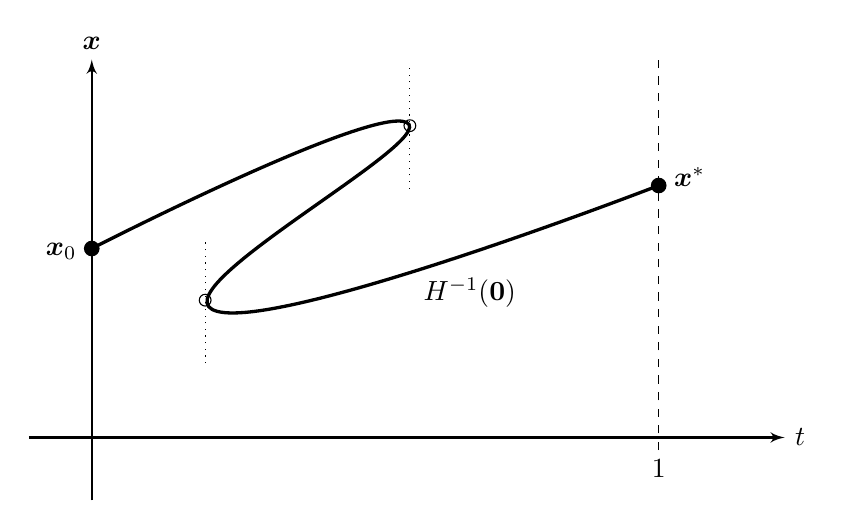
\begin{tikzpicture}[
		p1/.style={circle,fill,inner sep=2pt},
		p2/.style={circle,draw,inner sep=1.5pt},
		>=latex',
		scale=0.8]
	%% axis
	\draw[thick,->] (-1,0) -- (11,0) node[right] {$t$};
	\draw[thick,->] (0,-1) -- (0,6) node[above] {$\bm{x}$};
	\draw[dashed] (9,-0.2) node[below] {$1$} -- (9,6);
	%% define path
	\draw[very thick] plot [smooth, tension=1] coordinates {(0,3) (5,5) (2,2) (9,4)};
	%% define beginning and end
	\node at (0,3) [p1, label={[left,xshift=-2pt,yshift=-4pt] $\bm{x}_0$}] {};
	\node at (9,4) [p1, label={[right,xshift=2pt,yshift=0pt] $\bm{x}^*$}] {};
	\node at (6,2.3) {$H^{-1}(\bm{0})$};
	%% define turning points
	\node at (5.05,4.95) [p2] {};
	\draw[dotted] (5.05,3.95) -- (5.05,5.95);
	\node at (1.8,2.18) [p2] {};
	\draw[dotted] (1.8,1.18) -- (1.8,3.18);
\end{tikzpicture}
\end{center}
\vspace{1em}
\end{figure}

In general, the homotopy path $H^{-1}(\bm{0})$ is not guaranteed to as well-behaved as suggested by \autoref{fig:turningPoints}. It might feature multidimensional segments, bifurcations, dead ends or spirals. For path tracking to be well-defined, the homotopy path $H^{-1}(\bm{0})$ must include a smooth branch $\mathcal{H}^0$ through $(\bm{x}_0,0)$ that is almost everywhere one-dimensional, with only isolated transversals of auxiliary path segments. A corresponding illustration is provided in \autoref{fig:shapes}.

\begin{figure}[tbh]
\vspace{1em}
\caption{Possible Shapes of Homotopy Path}
\label{fig:shapes}
\vspace{1em}
\begin{minipage}{0.49\textwidth}
\begin{center}
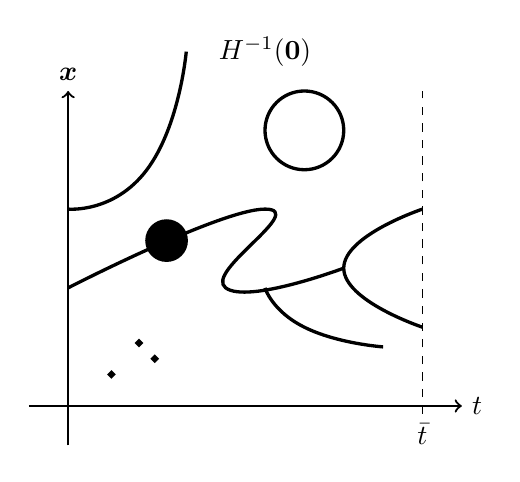
\begin{tikzpicture}[scale=0.5]
	%% axis
	\draw[thick,->] (-1,0) -- (10,0) node[right] {$t$};
	\draw[thick,->] (0,-1) -- (0,8) node[above] {$\bm{x}$};
	\draw[dashed] (9,-0.2) node[below] {$\bar{t}$} -- (9,8);
	%% define path
	\node at (5,9) {$H^{-1}(\bm{0})$};
	\draw[very thick] plot [smooth, tension=1] coordinates {(0,3) (5,5) (4,3) (7,3.5)};
	\draw[very thick] plot [smooth, tension=1] coordinates {(9,5) (7,3.5) (9,2)};
	\draw[very thick] plot (6,7) circle[radius=1];
	\filldraw[very thick] plot (1.1,0.8) circle[radius=0.05];
	\filldraw[very thick] plot (1.8,1.6) circle[radius=0.05];
	\filldraw[very thick] plot (2.2,1.2) circle[radius=0.05];
	\draw[very thick] plot [smooth, tension=1] coordinates {(5,3) (6,2) (8,1.5)};
	\spiral[very thick](5.3,1.3)(45:4:1);
	\draw[very thick] plot [smooth, tension=1] coordinates {(0,5) (2,6) (3,9)};
	\filldraw[very thick] plot (2.5,4.2) circle[radius=0.5];
\end{tikzpicture} \\
Path tracking infeasible. \\ \null
\end{center}
\end{minipage}
\hfill
\begin{minipage}{0.49\textwidth}
\begin{center}
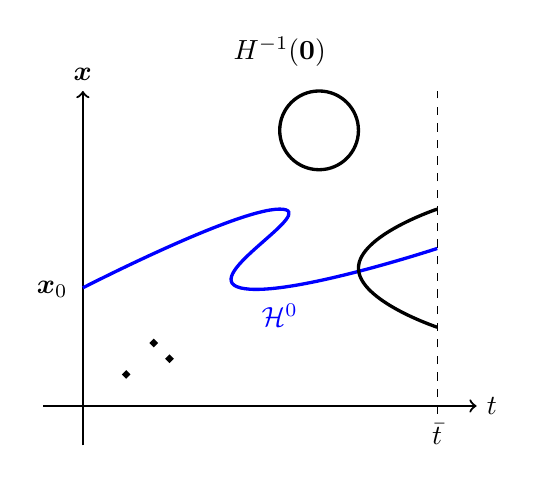
\begin{tikzpicture}[scale=0.5]
	%% axis
	\draw[thick,->] (-1,0) -- (10,0) node[right] {$t$};
	\draw[thick,->] (0,-1) -- (0,8) node[above] {$\bm{x}$};
	\draw[dashed] (9,-0.2) node[below] {$\bar{t}$} -- (9,8);
	%% define path
	\node at (5,9) {$H^{-1}(\bm{0})$};
	\node[blue] at (5,2.3) {$\mathcal{H}^0$};
	\draw[very thick, blue] plot [smooth, tension=1] coordinates {(0,3) (5,5) (4,3) (9,4)};
	\node at (0,3) [label={[left,xshift=-2pt,yshift=-4pt] $\bm{x}_0$}] {};
	\draw[very thick] plot [smooth, tension=1] coordinates {(9,5) (7,3.5) (9,2)};
	\draw[very thick] plot (6,7) circle[radius=1];
	\filldraw[very thick] plot (1.1,0.8) circle[radius=0.05];
	\filldraw[very thick] plot (1.8,1.6) circle[radius=0.05];
	\filldraw[very thick] plot (2.2,1.2) circle[radius=0.05];
\end{tikzpicture} \\
Path tracking feasible along \\ smooth branch $\mathcal{H}^0$ (blue).
\end{center}
\end{minipage}
\vspace{1em}
\end{figure}


Luckily, Sard's Theorem quarantees that \emph{almost all} systems of equations are well-behaved. If the system of interest happens not to be well-behaved, any random perturbation with continuous support will make the system well-behaved with probability one.




\section{Predictor-Corrector Procedure}


\begin{figure}[tbh]
\vspace{1em}
\caption{Predictor-Corrector Procedure}
\label{fig:predictorCorrector}
\begin{center}
\begin{tikzpicture}[
		p1/.style={circle,fill,inner sep=2pt}, 
		p2/.style={circle,draw,inner sep=1.5pt},
		p3/.style={circle,draw,inner sep=1pt},
		>=latex']
	%% define path
	\draw[very thick] plot [smooth, tension=1] coordinates {(0,0) (4,5) (10,2)};
	\node[below] at (10,2) {$H(\bm{y})=\bm{0}$};
	%% define points
	\node (yi) at (0.78,2) [p1, label={[below right,xshift=2pt] $\bm{y}_k$}] {};
	\node (yi0) at (4,8) [p2, label={[above left,xshift=2pt,yshift=-2pt] $\bm{y}_k^0$}] {};
	\node (yi0x) at (4.7,8.7) {};
	%(5,7.5)
	\node (yi1) at (5,7) [p3, label={[below left,xshift=-2pt,yshift=4pt] \footnotesize $\bm{y}_k^1$}] {};
	\node (yi1x) at (5.85,7.5) {};
	\node (yi2) at (5.4,6.2) [p3, label={[left,xshift=-2pt,yshift=-2pt] \footnotesize $\bm{y}_k^2$}] {};
	\node (yi2x) at (6.3,6.4) {};
	\node (yi3) at (5.5,5.8) [p3, label={[left,xshift=-2pt,yshift=-4pt] \footnotesize $\bm{y}_k^3$}] {};
	\node (yi3x) at (6.4,5.8) {};
	\node (yi4) at (5.5,5.3) {};
	\node (yin) at (5.4,5.3) {};
	\node (yj) at (5.3,5) [p1, label={[below,xshift=-4pt,yshift=-6pt] $\bm{y}_{k+1}$}] {};
	\node (yj0) at (9,4.1) [p2, label={[right,yshift=-2pt] $\bm{y}_{k+1}^0$}] {};
	%% define arrows
	\draw[->,thick] (yi) -- (yi0);
	\draw[decoration={brace,amplitude=10pt,raise=30pt},decorate] (yi) -- (yi0) node[midway,above left,xshift=-32pt,yshift=15pt] {\footnotesize $ds$};
	\draw[->] (yi0) -- (yi0x);
	\draw[->,thick,dotted] (yi0) -- (yi1);
	\draw[->] (yi1) -- (yi1x);
	\draw[->,thick,dotted] (yi1) -- (yi2);
	\draw[->] (yi2) -- (yi2x);
	\draw[->,thick,dotted] (yi2) -- (yi3);
	\draw[->] (yi3) -- (yi3x);
	\draw[->,thick,dotted] (yi3) -- (yi4);
	\draw[->,thick,dotted] (yin) -- (yj);
	\draw[->,thick] (yj) -- (yj0);
\end{tikzpicture}
\end{center}
\vspace{1em}
\end{figure}


Predictor-corrector procedures are \emph{the} standard tool to trace differentiable homotopy paths. As the name suggests, these are two-phase procedures, sequentially performing a prediction step and multiple correction steps. In the predictor step, the path at current point $\bm{y}_k$ is extrapolated along its tangent with step size $ds$. Afterwards, the predictor point $\bm{y}_k^0$ is refined by a number of Newton corrector steps. Corrector steps are performed orthogonally to current tangents until a new point $\bm{y}_{k+1}$ on the path is reached. Then, the step size is adapted and the two-step procedure is repeated, as illustrated in \autoref{fig:predictorCorrector}.

\textbf{Direction.} %
The homotopy path implied by $H(\bm{y})=0$ is defined up to its direction $\alpha \in \{1,-1\}$. In order to obtain the correct direction for path traversal, $\alpha$ is chosen such that the very first predictor step \emph{increases} $t$ and is held constant thereafter, except in the case of crossing a bifurcation point.


\begin{figure}[tbh]
\vspace{1em}
\caption{Simple Bifurcation}
\label{fig:simpleBifurcation}
\begin{center}
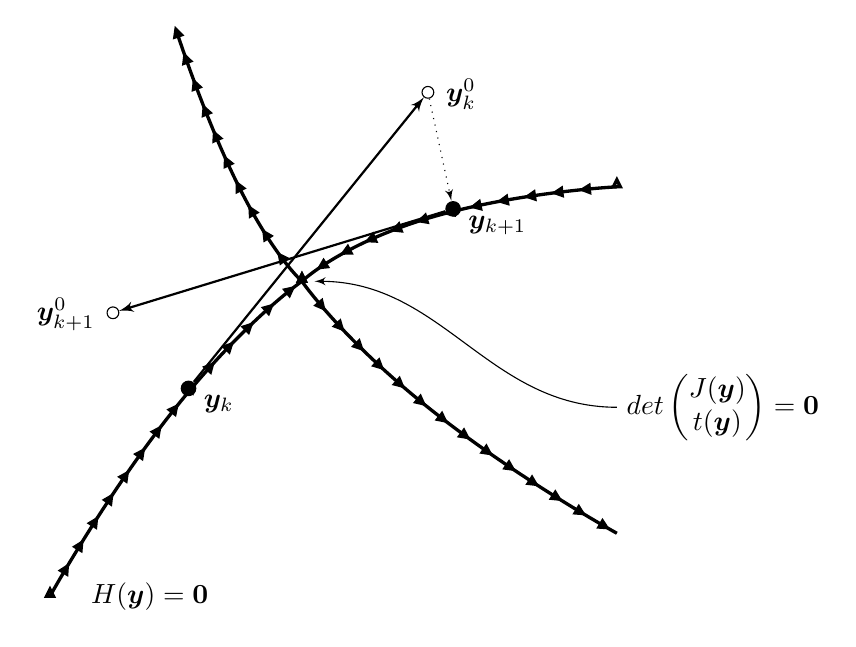
\begin{tikzpicture}[
		p1/.style={circle,fill,inner sep=2pt}, 
		p2/.style={circle,draw,inner sep=1.5pt},
		>=latex',
		scale=0.8]
	%% define path
	\draw[very thick,decoration=triangles,postaction={draw,decorate}] plot [smooth, tension=1] coordinates {(0,0) (2,3) (4,5)};
	\draw[very thick,decoration=triangles,postaction={draw,decorate}] plot [smooth, tension=1] coordinates {(9,6.5) (6,6) (4,5)};
	\draw[very thick,decoration=triangles,postaction={draw,decorate}] plot [smooth, tension=1] coordinates {(4,5) (3,6.5) (2,9)};
	\draw[very thick,decoration=triangles,postaction={draw,decorate}] plot [smooth, tension=1] coordinates {(4,5) (6,3) (9,1)};
	\node[right] at (0.5,0) {$H(\bm{y})=\bm{0}$};
	\draw[->] (9,3) node[right] {$det\begin{pmatrix}J(\bm{y})\\t(\bm{y})\end{pmatrix}=\bm{0}$} to[out=180,in=0] +(-4.8,+2);
	%% define points
	\node (yi) at (2.2,3.3) [p1, label={[below right,xshift=2pt,yshift=-2pt] $\bm{y}_k$}] {};
	\node (yi0) at (6,8) [p2, label={[right,xshift=3pt,yshift=-3pt] $\bm{y}_k^0$}] {};
	\node (yj) at (6.4,6.15) [p1, label={[below right,xshift=2pt,yshift=-2pt] $\bm{y}_{k+1}$}] {};
	\node (yj0) at (1,4.5) [p2, label={[left,xshift=-3pt,yshift=-3pt] $\bm{y}_{k+1}^0$}] {};
	%% define arrows
	\draw[->,thick] (yi) -- (yi0);
	\draw[->,dotted] (yi0) -- (yj);
	\draw[->,thick] (yj) -- (yj0);
\end{tikzpicture}%
\end{center}
\vspace{1em}
\end{figure}


\textbf{Bifurcation detection.} %
The principal branch of the homotopy path might be crossed by another branch at some point, as illustrated in \autoref{fig:simpleBifurcation}. These so-called simple bifurcations are singular points of the Jacobian matrix at which the direction of the path may be reversed \citep[chapter 8]{AllgowerGeorg1990}. In order to ensure continuation after the bifurcation, simple bifurcation points must be detected and, in case of a reversal of direction, the sign of direction $\alpha$ must be swapped. To detect bifurcations, the angle between consecutive predictor tangents is checked at each step. If the angle is close to 180\degree{} and the tangents point in almost opposite direction, the algorithm considers a bifurcation point with reversal of direction crossed. Specifically, the sign of $\alpha$ is swapped if
\begin{align*}
	\bigl[t(\bm{y}_k)\bigr]^T \cdot t(\bm{y}_{k-1}) \;<\; cos(\gamma_{\text{min}})
\end{align*}
with minimum angle $\gamma_{\text{min}}$ to classify changes in direction as bifurcation.

% AllgowerGeorg1990 method does not work well because there can also be bifurcations without reversal of direction!
%To detect bifurcations, the sign of the determinant of the augmented Jacobian is checked at each predictor-corrector step. If the sign changes between steps, i.e.\ if
%\begin{align*}
%	det \begin{pmatrix} J(\bm{y}_k) \\ t(\bm{y}_k) \end{pmatrix} \cdot det \begin{pmatrix} J(\bm{y}_{k-1}) \\ t(\bm{y}_{k-1}) \end{pmatrix} \;<\; 0,
%\end{align*}
%a bifurcation point was crossed and the direction of path traversal needs to be changed. 


\textbf{Predictor tangent.} %
At each point $\bm{y}_k$, the predictor tangent is computed based on a complete QR decomposition of the transpose $\bigl[ J(\bm{y}_k) \bigr]^T$ of the Jacobian at point $\bm{y}_k$. After successful QR decomposition, the tangent is essentially given by the last column of matrix $Q$, adjusted for the sign of the determinant of matrix $R$. Specifically, tangent $t(\bm{y}_k)$ is computed as
\begin{align*}
	t(\bm{y}_k) \;=\; \alpha \cdot \text{sign}(\det(R)) \cdot Q^{(n+1)}.
\end{align*}
Given step size $ds$ and tangent $t(\bm{y}_k)$, the predictor point $\bm{y}_k^0$ is given by
\begin{align*}
	\bm{y}_k^0 \;=\; \bm{y}_k + ds \cdot t(\bm{y}_k).
\end{align*}


\textbf{Newton correction.} %
The Newton correction is based on the Moore-Penrose pseudoinverse $\bigl[ J(\bm{y}_k^0) \bigr]^+$ of the Jacobian at predictor point $\bm{y}_k^0$. To be precise, the algorithm uses a Newton-Chord algorithm in which the pseudoinverse is only computed once at the prediction and used for all corrector steps. The pseudoinverse is computed based on a QR decomposition of $\bigl[ J(\bm{y}_k^0) \bigr]^T$ as
\begin{align*}
	\bigl[ J(\bm{y}_k^0) \bigr]^+ \;=\; Q \cdot \begin{pmatrix} (R^{(-t)})^{-1} \\ \bm{0} \end{pmatrix}
\end{align*}
where $R^{(-t)}$ denotes matrix $R$ without the row corresponding to differentiation with respect to $t$ within $J^T$. Given the pseudoinverse, corrector steps $l$ are performed analogously to Newton's method, i.e.\
\begin{align*}
	\bm{y}_k^l \;=\; \bm{y}_k^{l-1} - \bigl[ J(\bm{y}_k^0) \bigr]^+ \cdot H(\bm{y}_k^{l-1}),
\end{align*}
and iterated until either the tracking tolerance $H_{\text{tol}}$ is achieved or until failure (see next paragraph). To be conservative, the maximum norm is used to evaluate deviations from the path, i.e.\ the correction successfully terminates if
\begin{align*}
	\max \bigl\{ |H(\bm{y}_k^l)| \bigr\} \;<\; H_{\text{tol}}.
\end{align*}


\textbf{Newton robustness.} %
In order to ensure safe path traversal, the algorithm imposes a number of robustness requirements on the Newton correction. If one of the robustness criteria fails, i.e.\ if the convergence of the Newton correction is not ensured, the correction is aborted the predictor step is repeated with a decreased step size. 

The correction is considered unsuccessful if either (1) the number of corrector steps $L$ exceeds a threshold, (2) the distance $d_l$ of any corrector step relative to the predictor step size exceeds a threshold  or (3) the contraction of consecutive corrector steps, i.e.\ the ratio $\frac{d_l}{d_{l-1}}$ of distances exceeds a threshold. (4) Finally, following \cite{Choietal1996}, the algorithm additionally requires that the determinant of the augmented Jacobian does not change too much in the correction. Specifically, the correction is also considered unsuccessful if
\begin{align*}
	\left| \; \frac{ det \begin{pmatrix} J(\bm{y}_k^L) \\ t(\bm{y}_k) \end{pmatrix} }{ det \begin{pmatrix} J(\bm{y}_k) \\ t(\bm{y}_k) \end{pmatrix} } \right| \quad>\quad \bar{\Delta}_J
	\qquad\qquad\text{ or }\qquad\qquad
	\left| \; \frac{ det \begin{pmatrix} J(\bm{y}_k^L) \\ t(\bm{y}_k) \end{pmatrix} }{ det \begin{pmatrix} J(\bm{y}_k) \\ t(\bm{y}_k) \end{pmatrix} } \right| \quad<\quad \frac{1}{\bar{\Delta}_J}
\end{align*}
for a given maximum change $\bar{\Delta}_J > 0$. This robustness requirements prevents accidental ``path jumping'' to a different nearby segment illustrated in \autoref{fig:pathJumping}. When converging to a different path, the Jacobian typically changes so much that the correction is not accepted.


\begin{figure}[tbh]
\vspace{1em}
\caption{Path Jumping}
\label{fig:pathJumping}
\begin{center}
\begin{tikzpicture}[
		p1/.style={circle,fill,inner sep=2pt}, 
		p2/.style={circle,draw,inner sep=1.5pt},
		>=latex',
		scale=0.8]
	%% define path
	\draw[very thick] plot [smooth, tension=1] coordinates {(0,0) (4,3) (10,3)};
	\draw[very thick] plot [smooth, tension=1] coordinates {(2,9) (4,6) (10,6)};
	\node[above] at (10,4) {$H(\bm{y})=\bm{0}$};
	%% define points
	\node (yi) at (2,2.1) [p1, label={[below right,xshift=2pt,yshift=-2pt] $\bm{y}_k$}] {};
	\node (yi0) at (5,4.6) [p2, label={[right,xshift=3pt,yshift=-3pt] $\bm{y}_k^0$}] {};
	\node (yj) at (5.1,5.7) [p1, label={[above,xshift=2pt,yshift=2pt] $\bm{y}_{k+1}$}] {};
	%% define arrows
	\draw[->,thick] (yi) -- (yi0);
	\draw[->,dotted] (yi0) -- (yj);
\end{tikzpicture}
\end{center}
\vspace{1em}
\end{figure}


\textbf{Step size adaption.} %
After each predictor-corrector iteration, the step size is adjusted according to the performance of the Newton correction. In case of unsuccessful correction, the step size is reduced by a deflation factor $f_{\text{defl}} < 1$. In case of successful but slow correction, the step size is held constant. And in case of successful and fast correction, the step size is increased by an inflation factor $f_{\text{infl}} > 1$. The speed of correction is considered fast if less than ten corrector steps were performed until convergence.


\textbf{Convergence.} %
Two cases are distinguished. First, if $\bar{t} < \infty$, homotopy continuation is considered converged when $|t-\bar{t}| < t_{\text{tol}}$. Second, if $\bar{t} = \infty$, homotopy continuation is considered converged when the change in $\bm{x}$ between consecutive predictor-corrector steps relative to the step size falls below a tolerance level $x_{\text{tol}}$. To be conservative, the maximum norm is used to measure differences in $\bm{x}$. For further generality, one can define a transformation function $f: \R^{n+1} \rightarrow \R^m$ and consider changes in $f(\bm{x})$ for convergence.%
\footnote{%
This is particularly useful if the homotopy function is parameterized in for example logarithms of $\bm{x}$ or some other unbounded transformation.} %
Specifically, the algorithm reports convergence if 
\begin{align*}
	\max \Biggl\{ \frac{ \bigl| f(\bm{x})_k - f(\bm{x})_{k-1} \bigr| }{ ds } \Biggr\} \quad<\quad x_{\text{tol}}.
\end{align*}
In order not to impede performance, the algorithm checks for convergence in $\bm{x}$ only if the current step size is equal to the maximum step size, indicating the path has been relatively smooth for many consecutive steps. 






% ============================================ %
% ++++++++++++++++ LITERATURE ++++++++++++++++ %
% ============================================ %

\addcontentsline{toc}{section}{References}
\bibliography{literature}


\end{document}
